\documentclass{article}
\usepackage{enumitem}
\usepackage{graphicx}
\usepackage{float}
\usepackage{array}


\usepackage{geometry}
 \geometry{
 a4paper,
 left=20mm,
 right=20mm
 }


\newlist{legal}{enumerate}{10}
\setlist[legal]{label*=\arabic*.}

\begin{document}
	\begin{figure}
  	
\includegraphics[width=\linewidth]{./images/Logo-PoliMi.jpg}
	\end{figure}
\title{\textbf{RASD}}
\author{Paolo Romeo, Andrea Scotti, Francesco Staccone}
\date{AY 2018-2019}
\maketitle{}
\newpage
\textbf{Table of contents}
	\begin{legal}
 	\item Introduction
  		\begin{legal}
    		\item Purpose
		\item Scope
		\item Definitions, acronyms, abbreviations
		\item Reference documents
		\item Overview	
  		\end{legal}
	\item Overall Description
  		\begin{legal}
    		\item Product perspective
		\item Product functions
		\item User characteristics
		\item Constraints
		\item Assumptions and dependencies
  		\end{legal}
	\item Specific requirements
  		\begin{legal}
    		\item External interface requirements
		\item Functional requirements
		\item Performance requirements
		\item Design constraints
		\item Software system attributes
		\item Other requirements
  		\end{legal}
	\item Formal analysis using Alloy
  	\item Effort spent
	\item References
	\end{legal}
\newpage
	\begin{legal}\bfseries
 	\item Introduction \\
  		\begin{legal}
    		\item Purpose\\
		\\
		{\normalfont The purpose of this document is to fully describe the TrackMe application in terms of goals, functions, requirements and constraints of the system.}
		\\
		\item Scope\\
			\begin{legal}
    			\item Description of the given problem \\
			\item Goals \\
			{\normalfont
				\begin{itemize}
				\item G1) Third parties can monitor the position and the health status of the individuals. \\
				\item G2) Third parties can access the anonymized data of the groups of individuals.\\
				\item G3) The user can accept or refuse the requests concerning the treatment of his/her personal data by the third parties.\\
				\item G4) The third party can subscribe to new data and receive them as soon as they are produced.\\
				\item G5) The user can be recognized by providing a form of identification.\\
				\item G6) The third party can be recognized by providing a form of identification. \\
				\item G7) The user can check the position of the runners at any time during a race.\\
				\item G8) When the health status of the user is in danger, an SOS is launched and an ambulance is sent to the user’s current position.\\
				\item G9) A user can participate to the available races. \\
				\item G10) A third party can organize a race and define the path for the run.\\
				\end{itemize}
				}
			\end{legal}
		\item Definitions, acronyms, abbreviations\\
		\item Reference documents\\
		\item Overview\\
		\end{legal}
	
		
    		
		
	
\newpage
 	\item {Overall description}
  		\begin{legal}
    		\item Product perspective\\
			\begin{figure}[H]
  			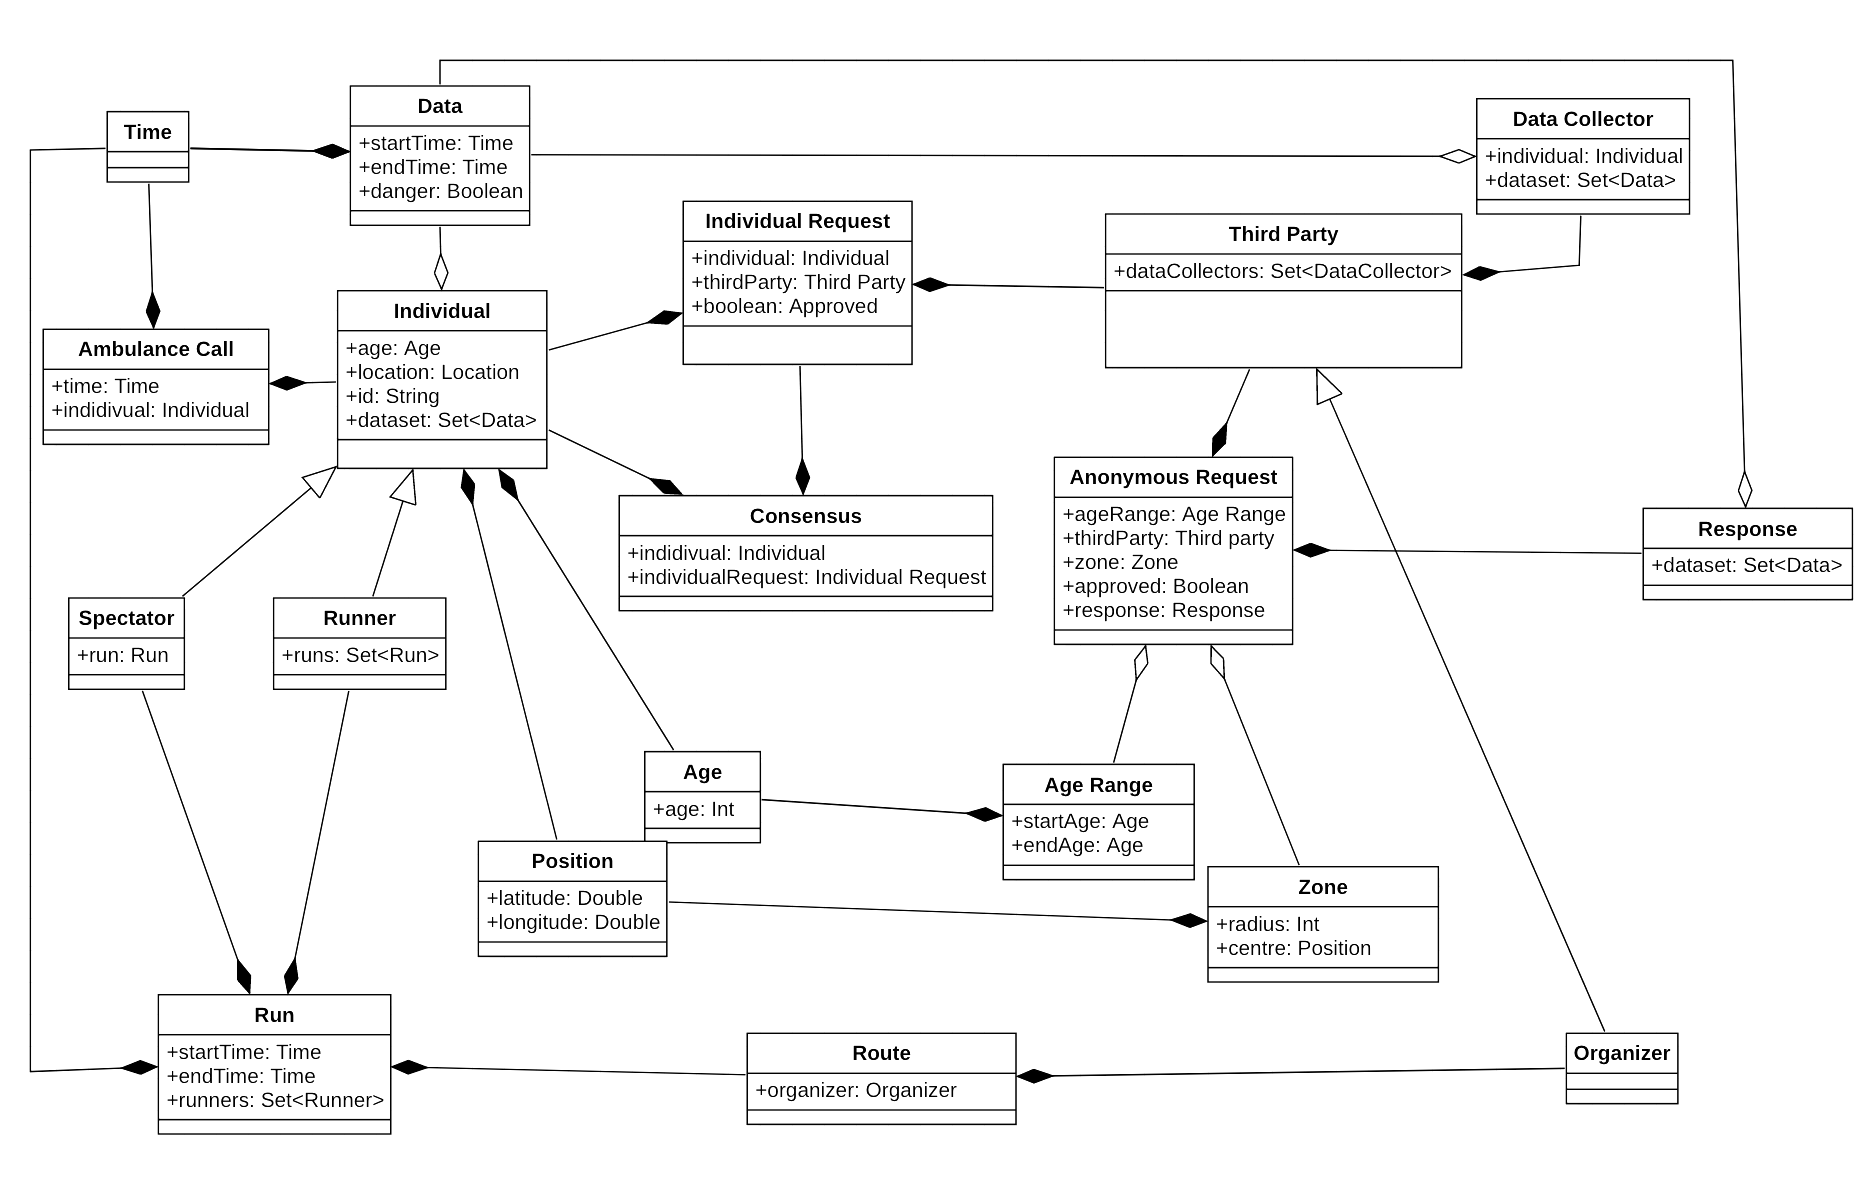
\includegraphics[width=\linewidth]{./images/UML1-0.png}
			\end{figure}
		\item Product functions \\
		\item User characteristics \\
		\item Constraints \\
		\item Assumptions and dependencies \\
			\begin{legal}
    			\item Text assumptions\\
    			{\normalfont
				\begin{itemize}
					\item User can choose to disable AUTOMATEDSOS service in preferences
					\item A SOS is sent through an SMS which contains the coordinates of the user's position.
					\item If the user is not able to connect the device, he can contact the TrackMe assistance by calling a specific number.
					\item When a user signs up to TrackMe he accpets also to treatment of his data for AUTOMATEDSOS
					\item The user can give up to the consensus to a third party.
				\end{itemize}}
			\item Domain assumptions \\
			{\normalfont
				\begin{itemize}
				\item D1) The measurements of the health status parameters of the individuals are supposed to be reliable.  \\
				\item D2) The position of the individuals is supposed to be reliable.\\
				\item D3) The data acquired from the user’s devices are sent to the mobile application as soon as they are produced.\\
				\item D4) The identification data provided by the users are correct.\\
				\item D5) The identification data provided by the third parties are correct.\\
				\item D6) When an SOS is launched, an ambulance is sent to the position of the user linked to the account that raised the SOS itself. \\
				\item D7) The race takes place in an area with internet coverage and in a compliant track.\\
				\item D8) ?????
				\end{itemize}
			}
			\end{legal}
		\end{legal}
	
\newpage
	\item Specific requirements\\
  		\begin{legal}
		\item External interface requirements\\
			\begin{legal}
    			\item User interfaces \\
				\begin{legal}
    				\item Login or Sign Up 
				\begin{figure}[H]
				\centering
  				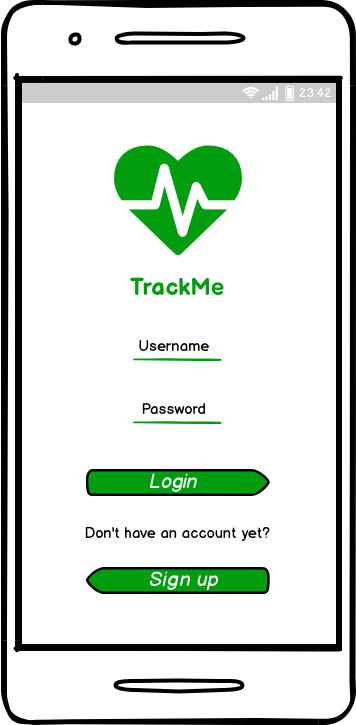
\includegraphics[scale=0.3]{./images/mockups/Login-Sign-up.png}
				\end{figure}
				\item Join a run 
				\begin{figure}[H]
				\centering
  				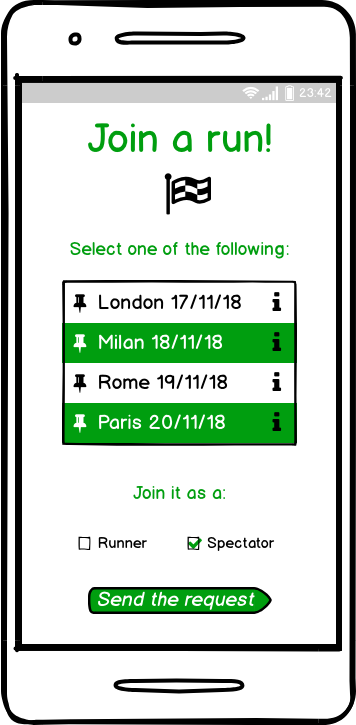
\includegraphics[scale=0.3]{./images/mockups/Join-a-run.png}
				\end{figure}
				\item Define the track of the run 
				\begin{figure}[H]
				\centering
  				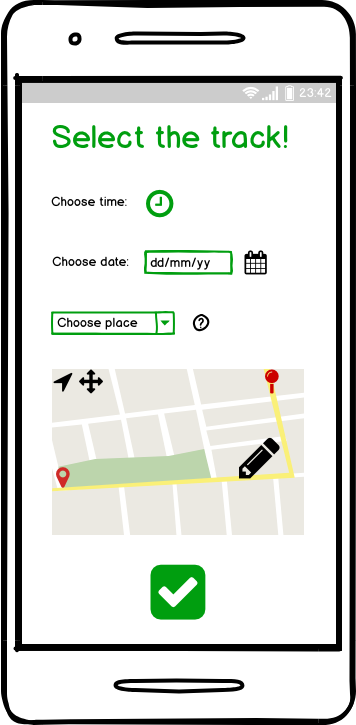
\includegraphics[scale=0.3]{./images/mockups/Path-definition.png}
				\end{figure}
				\item Individual request 
				\begin{figure}[H]
				\centering
  				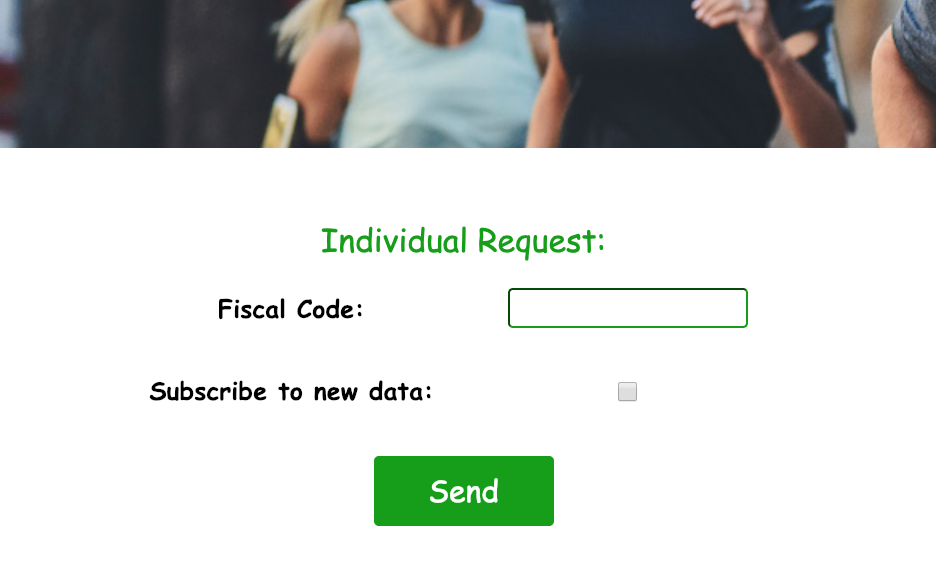
\includegraphics[scale=0.3]{./images/mockups/Individual-request.png}
				\end{figure}
				\item Group request 
				\begin{figure}[H]
				\centering
  				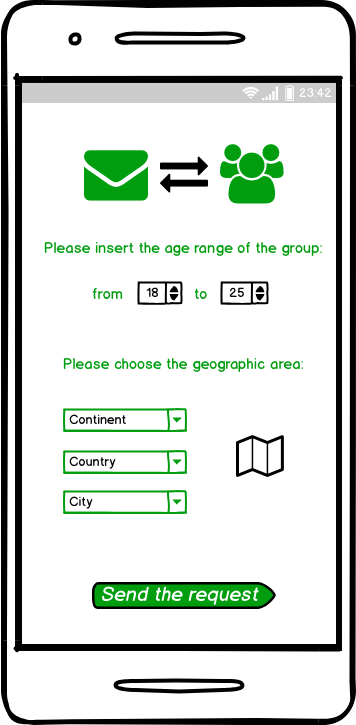
\includegraphics[scale=0.3]{./images/mockups/Group-request.png}
				\end{figure}
				
			\end{legal}
			\end{legal}

    		\item Functional Requirements\\
    		\begin{legal}\bfseries
    			\item Use Case Diagram
    			\begin{figure}[H]
			  	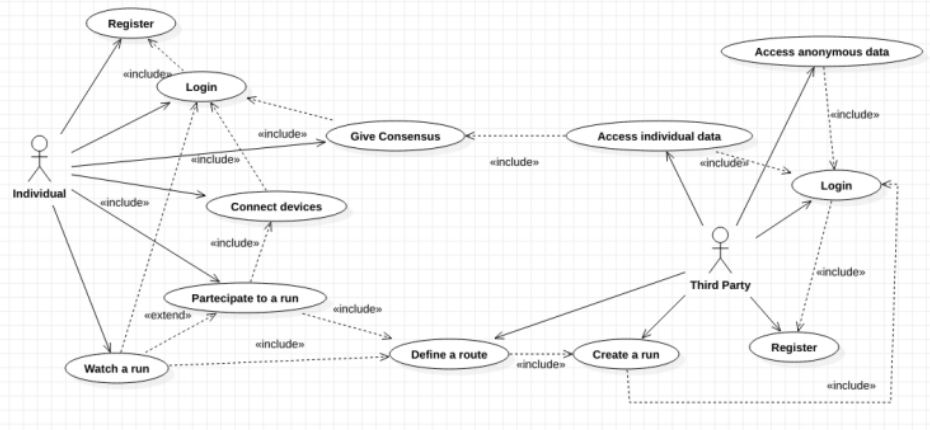
\includegraphics[width=\linewidth]{./images/usecase.png}
				\end{figure}
				\item Use Case Descriptions\\\\
				%SIGN UP
				\begin{tabular}{| m{3.5cm} | m{8cm}| }
				\hline
					Name & Sign up\\
				\hline
					Actor & Individual\\
				\hline
					Entry Conditions & Application installed
				on his device.\\
				\hline
					Event Flows & \begin{enumerate}
									\item The user opens the application.
									\item The user goes to the sign up section.
									
									\item The user gives all the necessary informations.
									\item The user chooses an username and a password.
									\item The user confirms his operations.
									\item The system save informations.
				\end{enumerate}\\
				\hline
					Exit Conditions & The user is successfully  registered and now he's able to log in.\\
				\hline
					Exceptions & \begin{enumerate}
									  \item The user is already registered.
									  \item The informations are incorrect or
									   missing.
				\end{enumerate}
				The user is notified and invited to try again.\\
				\hline
				\end{tabular}
				\\\\\\
				%LOGIN
				\begin{tabular}{| m{3.5cm} | m{8cm}| }
				\hline
					Name & Login\\
				\hline
					Actor & Individual\\
				\hline
					Entry Conditions & The user is previously successfully registered and has the application installed
				on his device.\\
				\hline
					Event Flows & \begin{enumerate}
									  \item The user opens the application.
									  \item The user goes to the login section.
									  \item The user inserts username and password.
									  \item The system checks if the credentials are correct.
				\end{enumerate}\\
				\hline
					Exit Conditions & The user is successfully logged in and he can access all the services. \\
				\hline
					Exceptions & The credentials are incorrect. The user is notified and invited to try again.\\
				\hline
				\end{tabular}\\\\\\
				%CONNECT A DEVICE
				\begin{tabular}{| m{3.5cm} | m{8cm}| }
				\hline
					Name & Connect a device\\
				\hline
					Actor & Individual\\
				\hline
					Entry Conditions & User already logged in.\\
				\hline
					Event Flows & \begin{enumerate}
									\item The user goes to the preference section.
									\item The user chooses to connect a device and then selects the right one.
				\end{enumerate}\\
				\hline
					Exit Conditions & The device is successfully connected to the application.\\
				\hline
					Exceptions & The system is not able to find or connect the device. The user is notified and invited to try again by reading carefully the connection instructions or to contact the help assistance of TrackMe.\\
				\hline
				\end{tabular}
				\\\\\\
				%WATCH A RUN
				\begin{tabular}{| m{3.5cm} | m{8cm}| }
				\hline
					Name & Watch a run\\
				\hline
					Actor & Individual\\
				\hline
					Entry Conditions & User already logged in.\\
				\hline
					Event Flows & \begin{enumerate}
									\item The user goes to the run section.
									\item The user chooses the run he wants to watch.
									\item The system screens a map with the route and the partecipants.
									\item The user can choose to watch statistics.
									\item If the user chooses to watch statistics the system provides him details about the run.
				\end{enumerate}\\
				\hline
					Exit Conditions & The user is able to follow a run.\\
				\hline
					Exceptions & There are no current runs. The user is notified with the list of incoming runs.\\
				\hline
				\end{tabular}
				\\\\\\
				%PARTECIPATE TO A RUN
				\begin{tabular}{| m{3.5cm} | m{8cm}| }
				\hline
					Name & Partecipate to a run\\
				\hline
					Actor & Individual\\
				\hline
					Entry Conditions & User already logged in and he has already given the consensus to the third party.\\
				\hline
					Event Flows & \begin{enumerate}
									\item The user goes to the run section.
									\item The system lists all available incoming runs which don't overlap with other user's runs.
									\item The user selects an incoming run.
									\item The system save the choice of the user in his calendar events.
				\end{enumerate}\\
				\hline
					Exit Conditions & The user is a official partecipant of the run and he will be notified some days before the run.\\
				\hline
					Exceptions & There are no available runs. The user is asked if he wants to be notified as soon as a new run is available.\\
				\hline
				\end{tabular}
				\\\\\\
				%GIVE CONSENSUS
				\begin{tabular}{| m{3.5cm} | m{8cm}| }
				\hline
					Name & Give consensus\\
				\hline
					Actor & Individual\\
				\hline
					Entry Conditions & User already logged in and a third party has requested access to user data.\\
				\hline
					Event Flows & \begin{enumerate}
									\item The user goes to the preference section.
									\item The user chooses to give or not the consensus to the third party.
									\item The system saves user's choice and sends it to the third party.
				\end{enumerate}\\
				\hline
					Exit Conditions & The third party can access user data if and only if the user gave the consensus.\\
				\hline
				\end{tabular}
				\\\\\\
				%CREATE A RUN
				\begin{tabular}{| m{3.5cm} | m{8cm}| }
				\hline
					Name & Create a run\\
				\hline
					Actor & Third Party\\
				\hline
					Entry Conditions & Third party logged in.\\
				\hline
					Event Flows & \begin{enumerate}
									\item The third party goes to the organize a run section.
									\item The system show to third party all the incoming events
									\item The third party chooses to create a run.
									\item The third party inserts all the relevant information except the route, it can be define later on.
									\item The system saves the event and update the calendar of incoming events of all the users.
				\end{enumerate}\\
				\hline
					Exit Conditions & The third party is ready to define a route and all the users are informed about the run.\\
				\hline 
					Exceptions & If the user hasn't given all the informations, he's asked to provide the missing ones.
					\\
				\hline
				\end{tabular}
				\\\\\\
				%ACCESS INDIVIDUAL DATA
				\begin{tabular}{| m{3.5cm} | m{8cm}| }
				\hline
					Name & Access individual data\\
				\hline
					Actor & Third Party\\
				\hline
					Entry Conditions & Third party logged in.\\
				\hline
					Event Flows & \begin{enumerate}
									\item The third party goes to the individual request section.
									\item The third party inserts the social security number of a person in order to request access of his/her data.
									\item The system forwards the request to the individual.
				\end{enumerate}\\
				\hline
					Exit Conditions & The user is notified about the request of the third party.\\
				\hline
					Exceptions & \begin{enumerate}
					\item The third party has already requested to access the data of the individual. In this case the third party is informed about the status of the individual's response.
					\item The social security number is not correct. The third party is notified and asked to try again.
					\end{enumerate}\\
				\hline
				\end{tabular}
				\\\\\\
				%ACCESS ANONYMOUS DATA
				\begin{tabular}{| m{3.5cm} | m{8cm}| }
				\hline
					Name & Access anonymous data\\
				\hline
					Actor & Third Party\\
				\hline
					Entry Conditions & Third party logged in.\\
				\hline
					Event Flows & \begin{enumerate}
									\item The third party goes to the group request section.
									\item The third party inserts the values of attributes of the the group of which is interested in.
									\item The system checks if the group is big enough to guarantee anonymity.
									\item The system will send the data to third party as soon as they are ready.
				\end{enumerate}\\
				\hline
					Exit Conditions & The third party has got access to the data of the interested group.\\
				\hline
					Exceptions & If the group is not big enough, the third party is notified and asked to try with other values of attributes.\\
				\hline
				\end{tabular}
				\\\\\\
    		\end{legal}
    		\item Software System Attributes \\
		\begin{legal}\bfseries
			\item Reliability
			\\\\
			{\normalfont The system is not fault tolerant, so it will be reliable according to its ability to avoid process crashes and to scale in case of numerous accesses.}
			\\
			\item Availability
			\\\\
			{\normalfont The system is not fault tolerant, so in case of failure it will not be available until the administrator will be able to reboot the system. So for this system availability is strictly correlated to maintainability.}
			\\
			\item Maintainability
			\\\\
			{\normalfont The code should be written in a way that favors the testability and the implementation of new functionalities.}
			\\
			\item Scalability
			\\\\
			{\normalfont The right choice of a PaaS allows the system to increase or decrease the level of allocated virtual resources at application or database on demand.}
			\\
			\item Portability
			\\\\
			{\normalfont The system front-end will be a web app, runnable on the majority of browsers but also natively on Android and IOS.}
			\\
			\item Safety
			\\\\
			{\normalfont The communication between the client and server is protected through a protocol such as HTTPS. The principal motivation is authentication of the accessed website and protection of the privacy and integrity of the exchanged data while in transit. It protects against man-in-the-middle attacks. The bidirectional encryption of communications between a client and server protects against eavesdropping and tampering of the communication. In practice, this provides a reasonable assurance that one is communicating without interference by attackers with the website that one intended to communicate with, as opposed to an impostor. }
			\\
			
			
		\end{legal}
		\end{legal}

	\end{legal}
\end{document}